\documentclass[11pt]{article}

%%%%%%%%%%%%%%Include Packages%%%%%%%%%%%%%%%%%%%%%%%%%%
\usepackage{xcolor}
\usepackage{mathtools}
\usepackage[a4paper, total={6in, 8in}, margin=1.25in]{geometry}
\usepackage{amsmath}
\usepackage{amssymb}
\usepackage{paralist}
\usepackage{rsfso}
\usepackage{amsthm}
\usepackage{wasysym}
\usepackage[inline]{enumitem}   
\usepackage{hyperref}
\usepackage{tocloft}
\usepackage{titlesec}
\usepackage{colortbl}
%%%%%%%%%%%%%%%%%%%%%%%%%%%%%%%%%%%%%%%%%%%%%%%%%%%%%%%%



\begin{document}
\Large \noindent \textbf{Physics 5C Discussion (Week 3)}\\
\normalsize
Department of Physics and Astronomy, UCLA\\
%\noindent TA: Jinyan Miao (jnmiu@ucla.edu)\\
%Office hours: Thursday 10-11 AM $\&$ 1-2 PM at PAB 2-429\\
%Tutoring center hours: Friday 2-3 PM at PAB 2-429 (Zoom room also available)\\
\noindent\rule{8cm}{0.4pt}\\

\noindent\textbf{Problem 1}:
Consider a parallel-plate capacitor, formed by two conducting plates that carry charges as shown. The electric field in between the plates is uniform (being the same everywhere, in both direction and magnitude). The magnitude of the electric field between the plates is 
\begin{align*}
|\vec{E}| = \frac{Q}{\epsilon_0 A}\,,
\end{align*}
with $A$ being the area of each of the plates and $Q$ being the amount of positive charge stored at the top plate.\\

\begin{center}
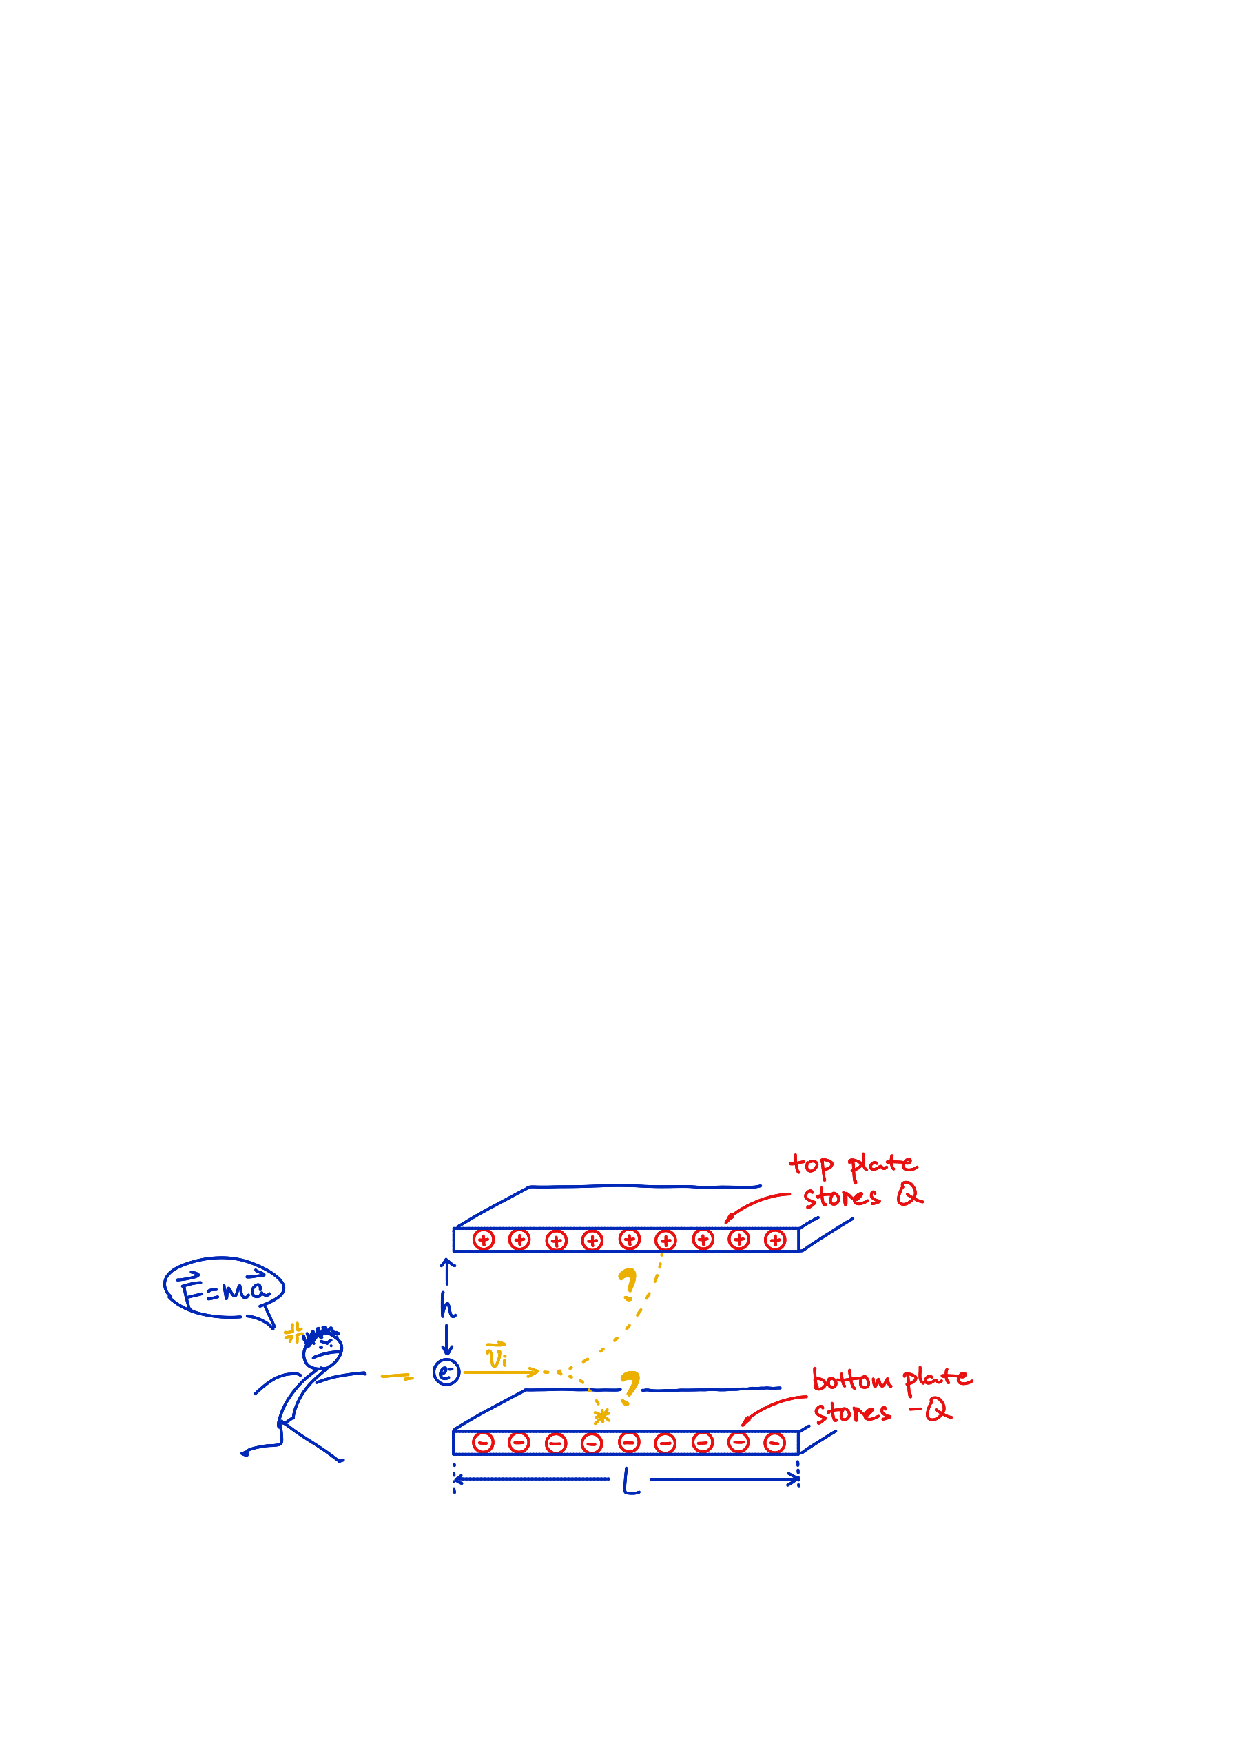
\includegraphics[scale=0.85]{capacitor}
\end{center}


\noindent\textbf{Part (a)} Based on the sign of the charges stored at the two plates, determine the direction of the electric field, and write down the vector form of the electric field $\vec{E} = (E_x,E_y)$ between the plates in terms of the variables $Q,\,A$ and the constant $\epsilon_0$. \\

\noindent \textbf{Part (b)} Now Jinyan throws an electron with charge $q$ into the region between the two plates. The electron experiences a force due to the electric field. 
%Assume $A = 1\,$m$^2$ is the area of each of the plates and $Q = 1$\,C. Recall that $\epsilon_0 = 8.9 \cdot 10^{-12}$\,Fm$^{-1}$. 
Compute the electric force that the electron experiences, write it in its vector form $\vec{F} = (F_x,\,F_y)$ in terms of the unknown variables $q,\,Q,\,A$ and the constant $\epsilon_0$.\\

\noindent \textbf{Part (c)} The electron (with mass $m$) enters the region with initial velocity $\vec{v}_i = (v_{0,x},0)$, at a position $h\,$ meters below the top plate. Each of the plates is $L$ meters long. Symbolically compute the minimal speed $v_{0,x}$ needed such that the electron can pass through the region without hitting either plate. Neglect gravity and friction.\footnote{Hint: This part is a Physics-5A type of problem, you can solve it using either conservation of energy (if acceleration $\vec{a}$ is not a constant) or kinematic equations (if $\vec{a}$ is a constant). Your answer should be in terms of $q,\,Q,\,m,\,L,\,h,\, A$ and $\epsilon_0$.}


\newpage
\noindent\textbf{Problem 2}: Now we revisit the problem on the week-2 worksheet again. 
\begin{center}
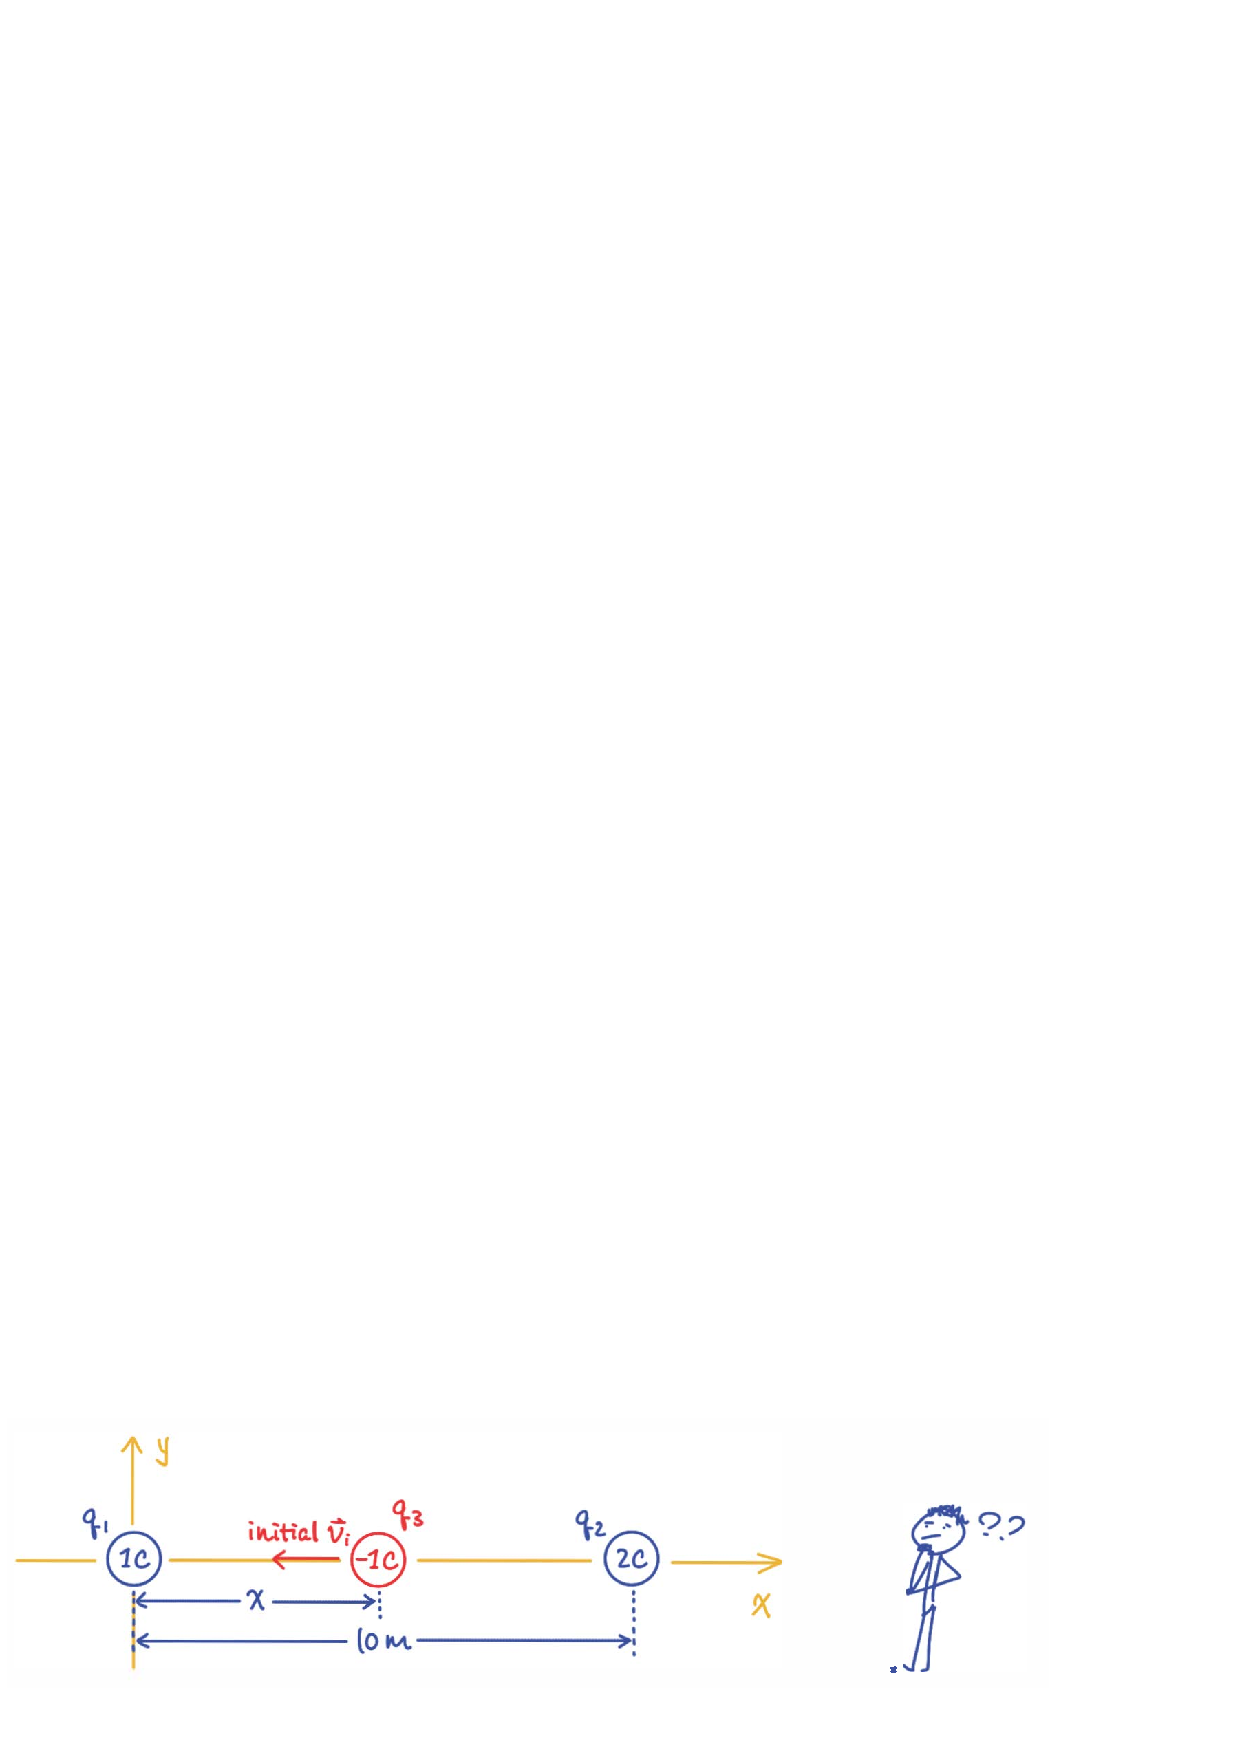
\includegraphics[scale=0.8]{lineChargeX}
\end{center}
\noindent $q_1 = 1\,$C is fixed at $\vec{x}_1 = (0,0)$\,m. \\
$q_2=2\,$C is fixed at $\vec{x}_2 =(10,0)$\,m. \\
$q_3=-1$\,C is initially between $q_1$ and $q_2$ on the $x$-axis with some initial velocity.\\
The Coulomb constant $k = 8.99 \cdot 10^9$\,Nm$^2$/C$^2$.\\

\noindent\textbf{Part (a)} Find the electric potential in the region between the two positive charges (that is, you neglect the negative charge in the middle, for this part). \\

\noindent\textbf{Part (b)} Find the electric potential energy of the negative charge $q_3$, when it is placed at $\vec{x} = (x,0)$ between $q_1$ and $q_2$.\\

\noindent\textbf{Part (c)} If $q_3$ is initially at $\vec{x} = (5,0)$\,m, with initial velocity $\vec{v} = (-1,0)$\,m/s. Will it be able to pass through the point where it experiences zero net force? \footnote{Hint: From the week-1 worksheet, $q_3$ experiences zero net force at $x = 4.14$\,m. Apply energy conservation to see whether $q_3$ has enough initial kinetic energy to overcome the potential energy difference between the starting location at $x=5$\,m and the target location at $x = 4.14$\,m.}


%
%\newpage
%\section*{Problem 1}
%Since we have positive charges on the top plate, and negative charges on the bottom plate, we expect the electric field lines to be going from the top to the bottom plate, straight down. Then we can write
%\begin{align*}
%\vec{E} = \left(0,\, -\frac{Q}{\epsilon_0 A}\right)\,.
%\end{align*}
%The force that the electron experiences upon entering the region is 
%\begin{align*}
%\vec{F} = q\vec{E} = \left(0,\, -\frac{qQ}{\epsilon_0 A}\right) = \left( 0,\, \frac{|q|Q}{\epsilon_0 A} \right)\,\text{N}\,.
%\end{align*}
%Notice that the negative sign from $q$ cancels the negative sign in the $y$-component of electric field, and thus the electron gets pulled upward. A key observation here is that the force acting on the electron is a constant force, it does not depend on where the electron is as long as it stays inside the region. This is a characteristic of charges moving inside a parallel-plate capacitor. \\
%
%Now since we have a constant force, the electron inside the capacitor will move under a constant acceleration, so we use kinematic equations (which require the assumption of having constant acceleration) to describe the motion of the electron. The acceleration of the electron when moving in the capacitor is, per Newton's Second Law, 
%\begin{align*}
%\vec{a} = \frac{\vec{F}}{m} = \left(0,\, \frac{|q|Q}{\epsilon_0 Am} \right)\,\text{m/s}^2\,.
%\end{align*}
%This is an acceleration straight up, so we expect to solve for something like an ``inverted" projectile motion (projectile motion has constant gravitational acceleration going down, resulting in a concave-down parabolic motion, now we have constant acceleration going up, resulting in a concave-up parabolic motion). We neglect gravity in this problem, and there is no friction, so $\vec{a}$ as computed above due to the electric force is the only acceleration that the electron experiences. Employ the kinematic equations, 
%\begin{align*}
%\Delta y = \frac{1}{2}a_y t^2 + v_{0,y} t\,,\qquad
%\Delta x = \frac{1}{2}a_x t^2 + v_{0,x} t\,.
%\end{align*}
%The electron wants to move up, there is a chance that it will hit the upper plate, and we want to prevent that from happening, so we want $\Delta y < 1$\,m when the electron exits the region. Therefore, we can first find out the time that the electron will reach $\Delta y = 1$, 
%\begin{align*}
%h=\Delta y = \frac{1}{2}a_y t^2 + v_{0,y}t = \frac{1}{2}\frac{|q|Q}{\epsilon_0 Am} t^2 \,,
%\end{align*}
%so we have
%\begin{align*}
%t = \sqrt{\frac{2h Am\epsilon_0}{|q|Q}}\,.
%\end{align*}
%That means, the electron should better be able to exit the region within $•$ seconds, so that it does not hit the top plate. To exit the region, we want $\Delta x = L$\,m because the plates are $L$ meters long, so 
%\begin{align*}
%L < \frac{1}{2}a_xt^2 + v_{0,x}t = v_{0,x}\sqrt{\frac{2h Am\epsilon_0}{|q|Q}} \,,
%\end{align*}
%from which we find that we want to have 
%$$v_{0,x} > \sqrt{\frac{|q|QL^2}{2hAm\epsilon_0}}\,.$$ 
%I just put the $L$ into the square-root to make it look nicer. Anything equivalent to this is correct. 
%
%
%\section*{Problem 2}
%The electric potential due to the charge $q_1$ on the left is 
%\begin{align*}
%V_1 = \frac{kq_1}{r}\,,
%\end{align*}
%with $r$ being the distance measured from charge $q_1$ at the origin. In the figure, this is denoted as $x$, so
%\begin{align*}
%V_1 = \frac{kq_1}{x}\,.
%\end{align*}
%Here we require $0<x<10$, otherwise we will need to put absolute value sign for $x$ because we want to measure the ``distance" from $q_1$, which is always positive. Now for $q_2$, 
%\begin{align*}
%V_2 = \frac{kq_2}{10-x}\,,
%\end{align*}
%and again, we require $0<x<10$. The electric potential anywhere in between $q_1$ and $q_2$ is thus
%\begin{align*}
%V = V_1 + V_2 = \frac{kq_1}{x} + \frac{kq_2}{10-x}\,.
%\end{align*}
%Sure, we can plug in the numbers, 
%\begin{align*}
%V = \left(\frac{8.99\cdot 10^9}{x} + \frac{2\cdot 8.99\cdot 10^9}{10-x}\right)\,\text{V}.
%\end{align*}
%The italicized $V$ is the electric potential, the normal font V is the unit voltage. To get more intuition about what this is, I can plot $V$ for $0<x<10$. In fact, let me plot 
%\begin{align*}
%V = \left(\frac{8.99\cdot 10^9}{|x|} + \frac{2\cdot 8.99\cdot 10^9}{|10-x|}\right)\,\text{V}
%\end{align*}
%such that you can also see what happens outside of $0<x<10$. 
%\begin{center}
%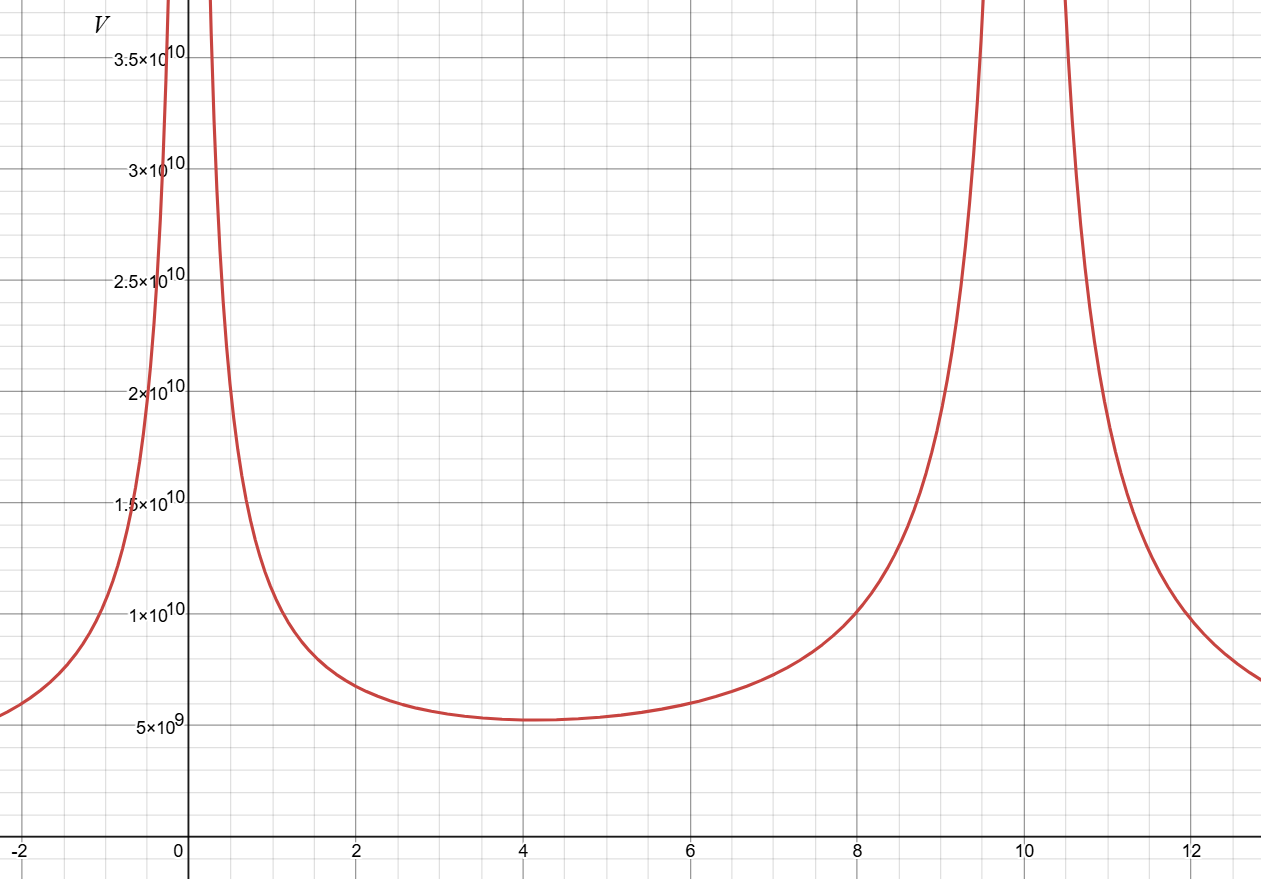
\includegraphics[scale=0.25]{V}
%\end{center}
%It looks like we have two big mountains at $x=0$ and $x=10$, with the one at $x=10$ slightly larger. This is exactly an analogy that you should be thinking about: If I put another positive charge in between $q_1$ and $q_2$, the positive charges will be oscillating in the region between $q_1$ and $q_2$, as if a spherical mass rolling around the trough of the two mountains. However, what we actually put here is a negative charge, so we should flip the ``mountains" upside down. The potential energy stored in the negative charge $q_3$ is 
%\begin{align*}
%U = q_3 V =(-1\,\text{C})\cdot V =\left(-\frac{8.99\cdot 10^9}{|x|} - \frac{2\cdot 8.99\cdot 10^9}{|10-x|}\right) \,\text{J}\,.
%\end{align*}
%If you plot $U$, you see that we get the inverted mountains, the inversion comes from the negative sign in $q_3$. Now the two inverted mountains are like big sinks on the sides, and the inverted trough becomes a small hill in the middle. \\
%\begin{center}
%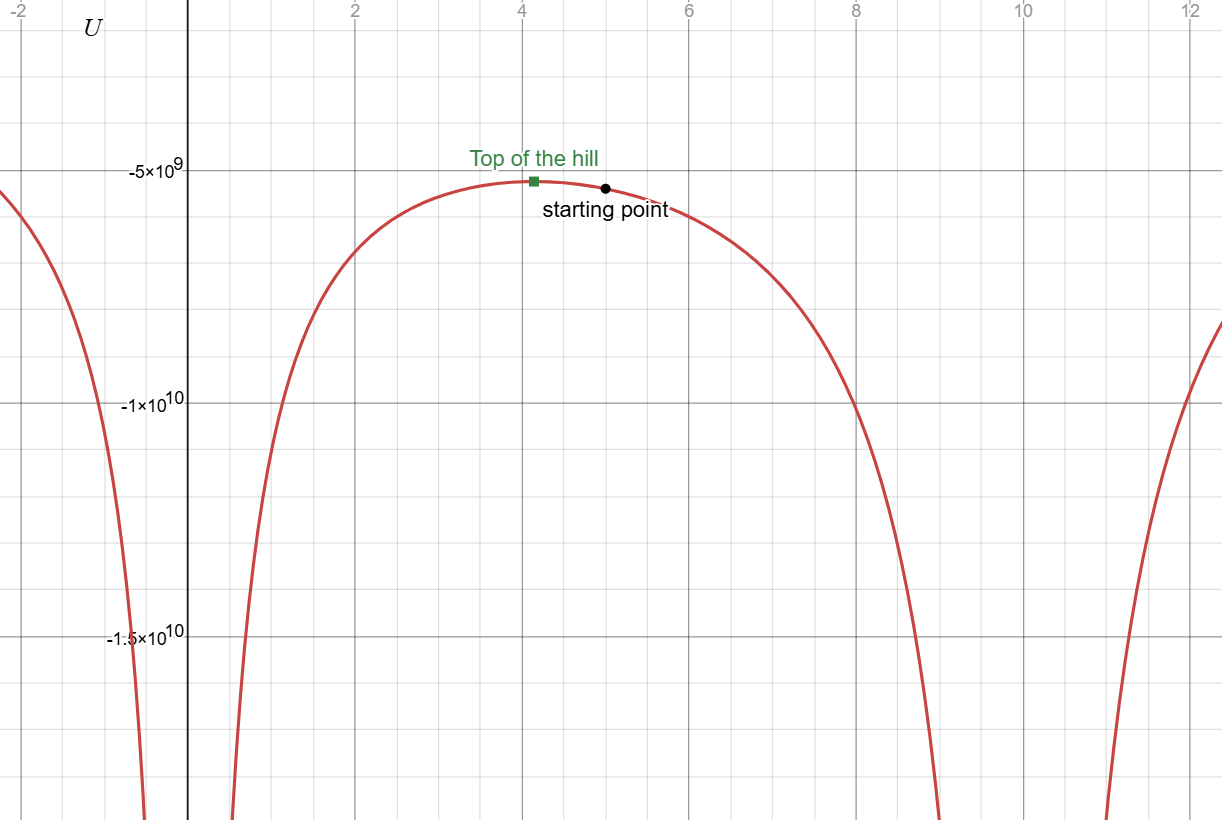
\includegraphics[scale=0.25]{U}
%\end{center}
%I have also labeled on the graph where $q_3$ starts its motion. Since it is initially moving to the left, it is initially ``climbing up a hill" in the middle. Depending on whether it can get to the top of the hill from the right, it will either roll to the left sink or roll to the right sink eventually. The top of the hill is in fact located at $x = 4.14$ which we found in week-2 discussion. Why? On the left of $x=4.14$, $q_3$ wants to accelerate to the left as the attraction due to the left charge $q_1$ is too strong; On the right of $x= 4.14$, $q_3$ wants to accelerate to the right; Same thing applies to the ``hill" picture. To see whether $q_3$ can ``get to the top of the hill," we use conservation of energy, 
%\begin{align*}
%\text{Initial Energy} &= \text{Final Energy}\,,\\
%\text{KE}_i+ \text{PE}_i &= \text{KE}_f + \text{PE}_f\,.
%\end{align*} 
%Our goal here is to see whether we have enough initial kinetic energy to overcome the potential energy difference between the initial point and the ``top of the hill." In other words, find out whether $q_3$ is going fast enough to the left initially to climb to the top of the hill. Therefore, we first compute the potential energy difference, 
%\begin{align*}
%\text{PE}_f& - \text{PE}_i = U(x=4.14)- U(x=5)\\
%&= \left(-\frac{8.99\cdot 10^9}{4.14} - \frac{2\cdot 8.99\cdot 10^9}{10-4.14}\right)-
%\left(-\frac{8.99\cdot 10^9}{5} - \frac{2\cdot 8.99\cdot 10^9}{10-5}\right) =1.5\cdot 10^8\,\text{J}\,.
%\end{align*}
%Ooof, this is a huge number. The amount of kinetic energy that we have at the beginning is only 
%\begin{align*}
%\text{KE}_i = \frac{1}{2}mv_{i,x}^2 = \frac{1}{2}\cdot (9.109 \cdot 10^{-31})\cdot (-1)^2 = 4.6\cdot 10^{-31}\,\text{J}\,,
%\end{align*}
%which is tiny. Therefore, there is not enough initial kinetic energy for $q_3$ to get to the top of the hill, and thus it will not pass through the point where it experiences zero force. It will eventually turn around, travel to the right, and hit the charge $q_2$ on the right.\\
%
%\begin{center}
%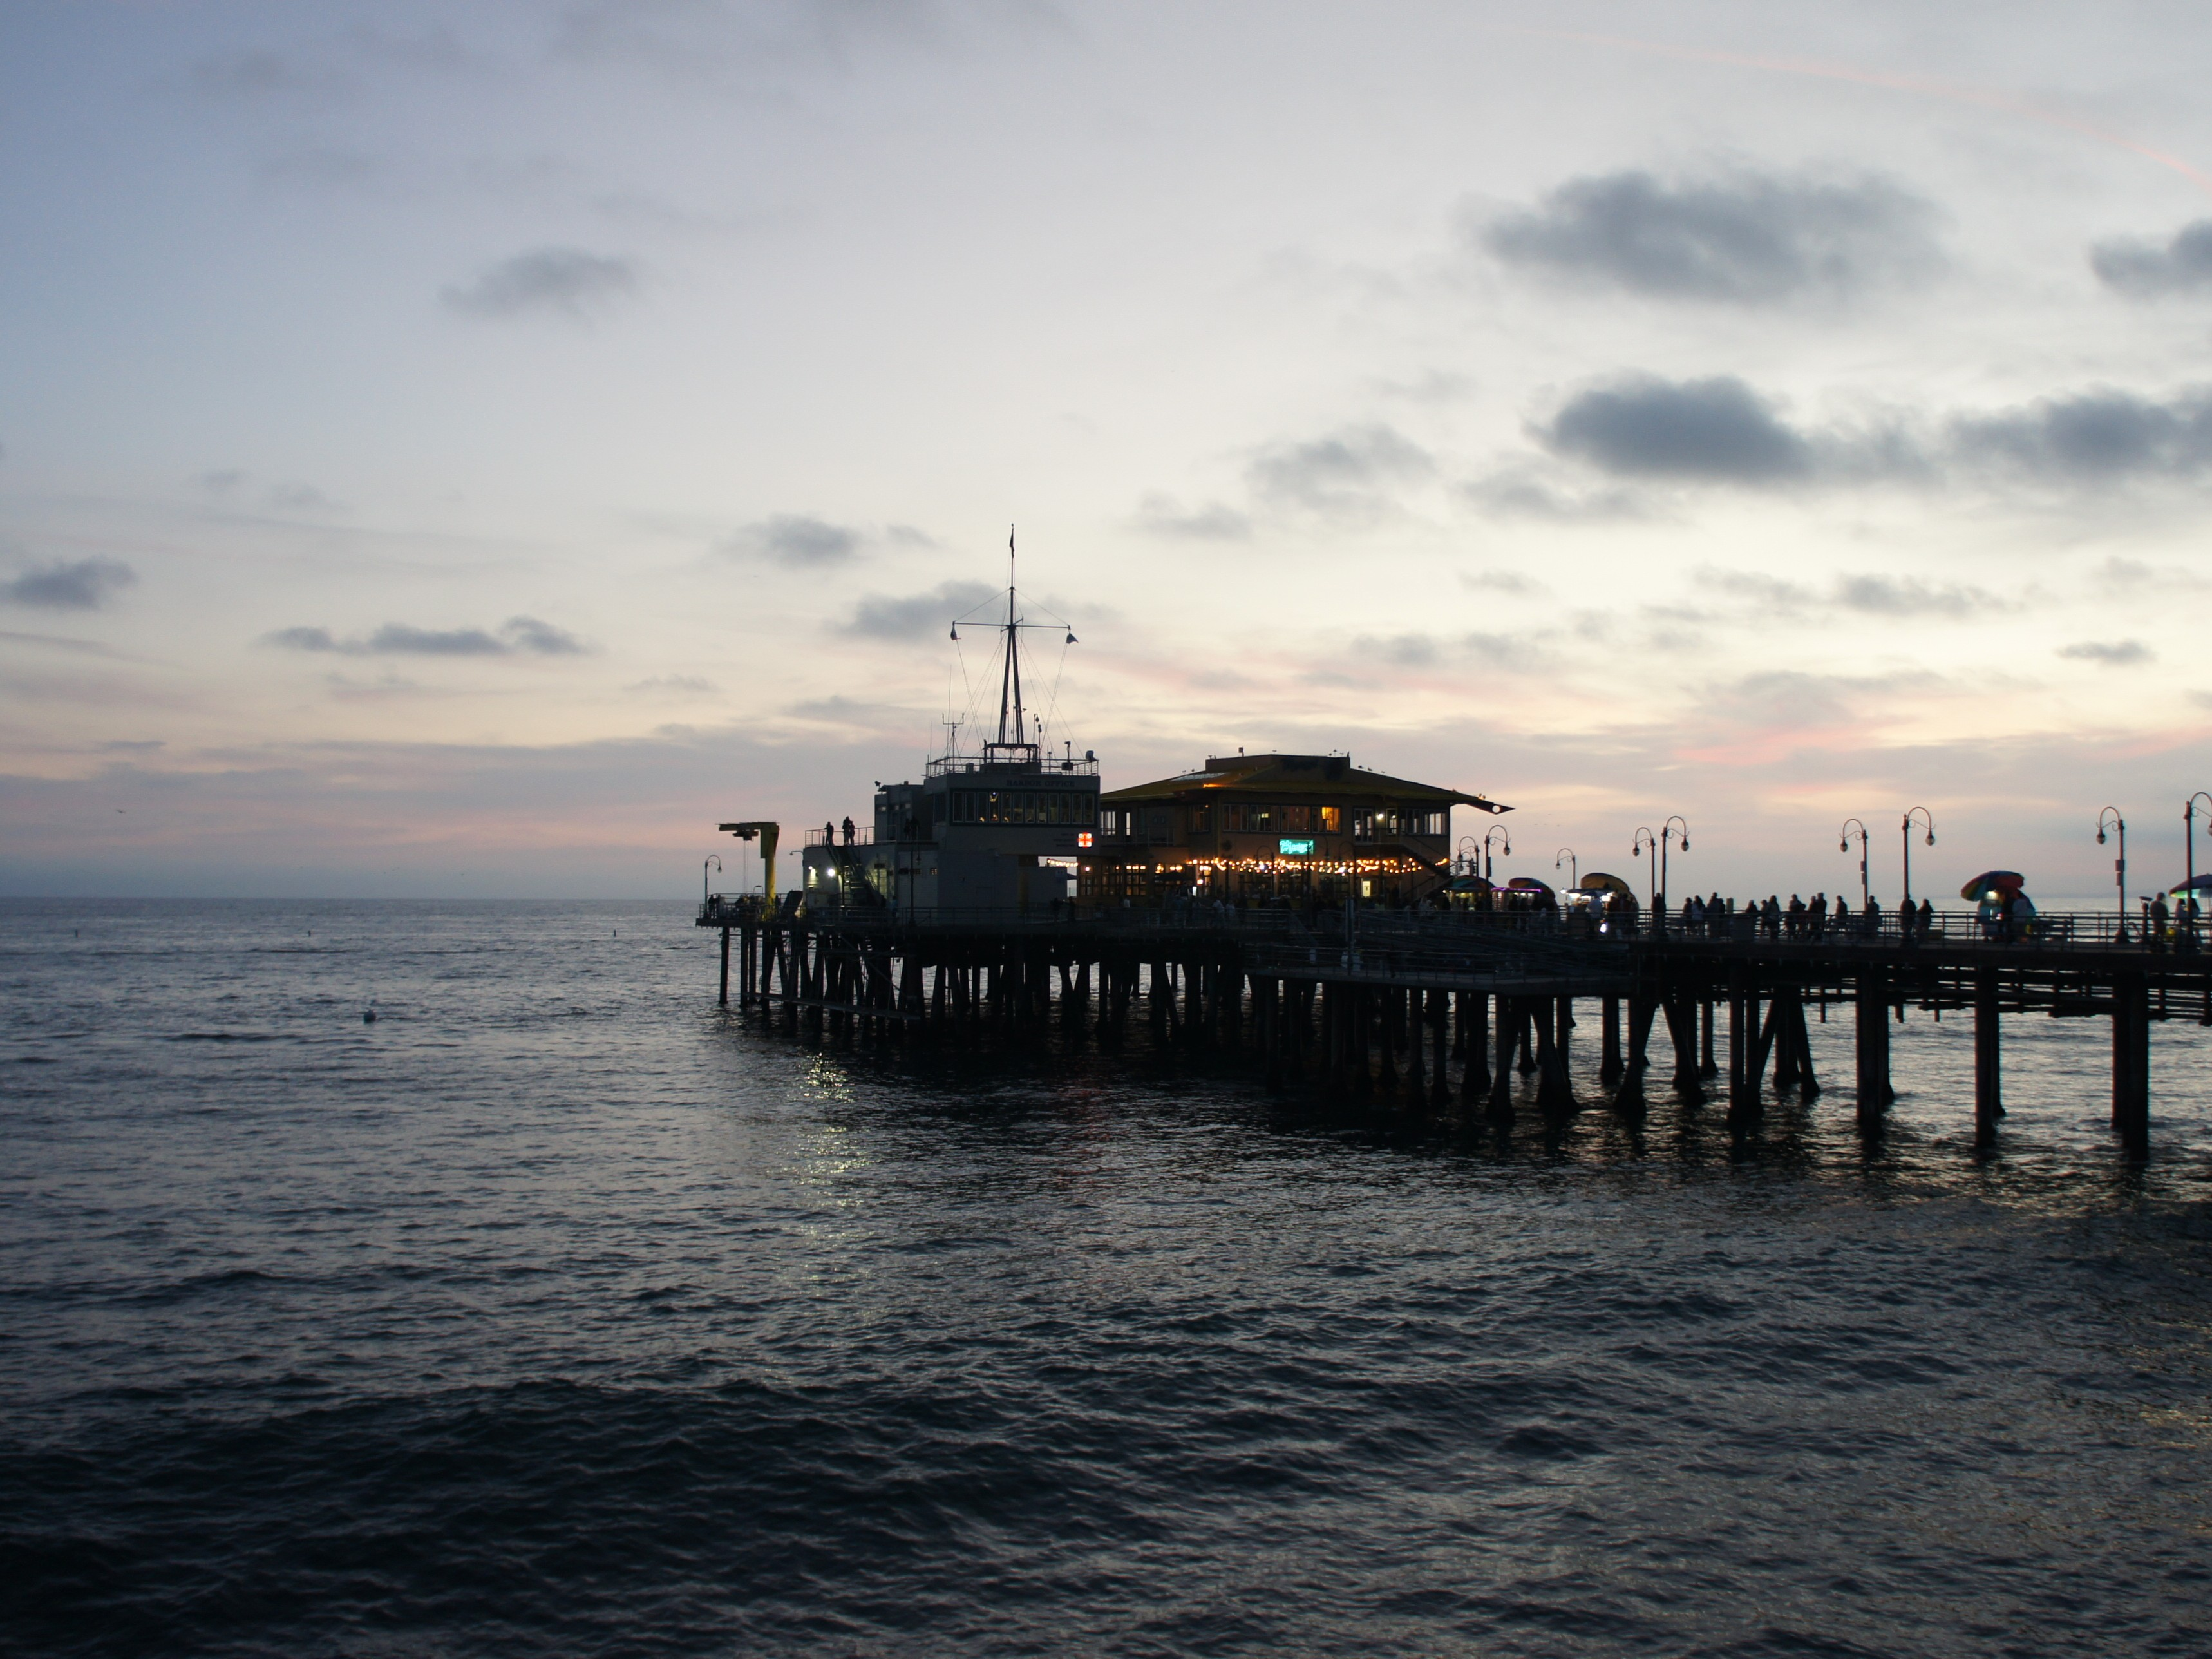
\includegraphics[scale=0.1]{DSC07127}\\
%\hfill\break
%The photo of this week is Santa Monica Pier :)
%\end{center}


\end{document}


